\subsection{VDB Implementation}

In this section the theory and implementation the VDB data structure is covered.

The VDB (Volumetric Dynamic B-tree) is an advanced data structure designed for efficient and flexible representation of sparse volumetric data. It is organized hierarchically, consisting of root nodes, internal nodes, and leaf nodes, each serving distinct purposes within the structure. This section begins by explaining in detail how VDB is structured, and it continues by going though the implementation of the data structure in the rendering engine.

\subsubsection{Data Structure}
VDBs are sparse, shallow trees with a fixed depth but expandable breadth, capable of covering an virutally infinite spatial domain. This design enables the VDB to efficiently manage large and complex datasets by adjusting the level of detail dynamically and minimizing memory usage.

\begin{figure}[H]
  \centering
  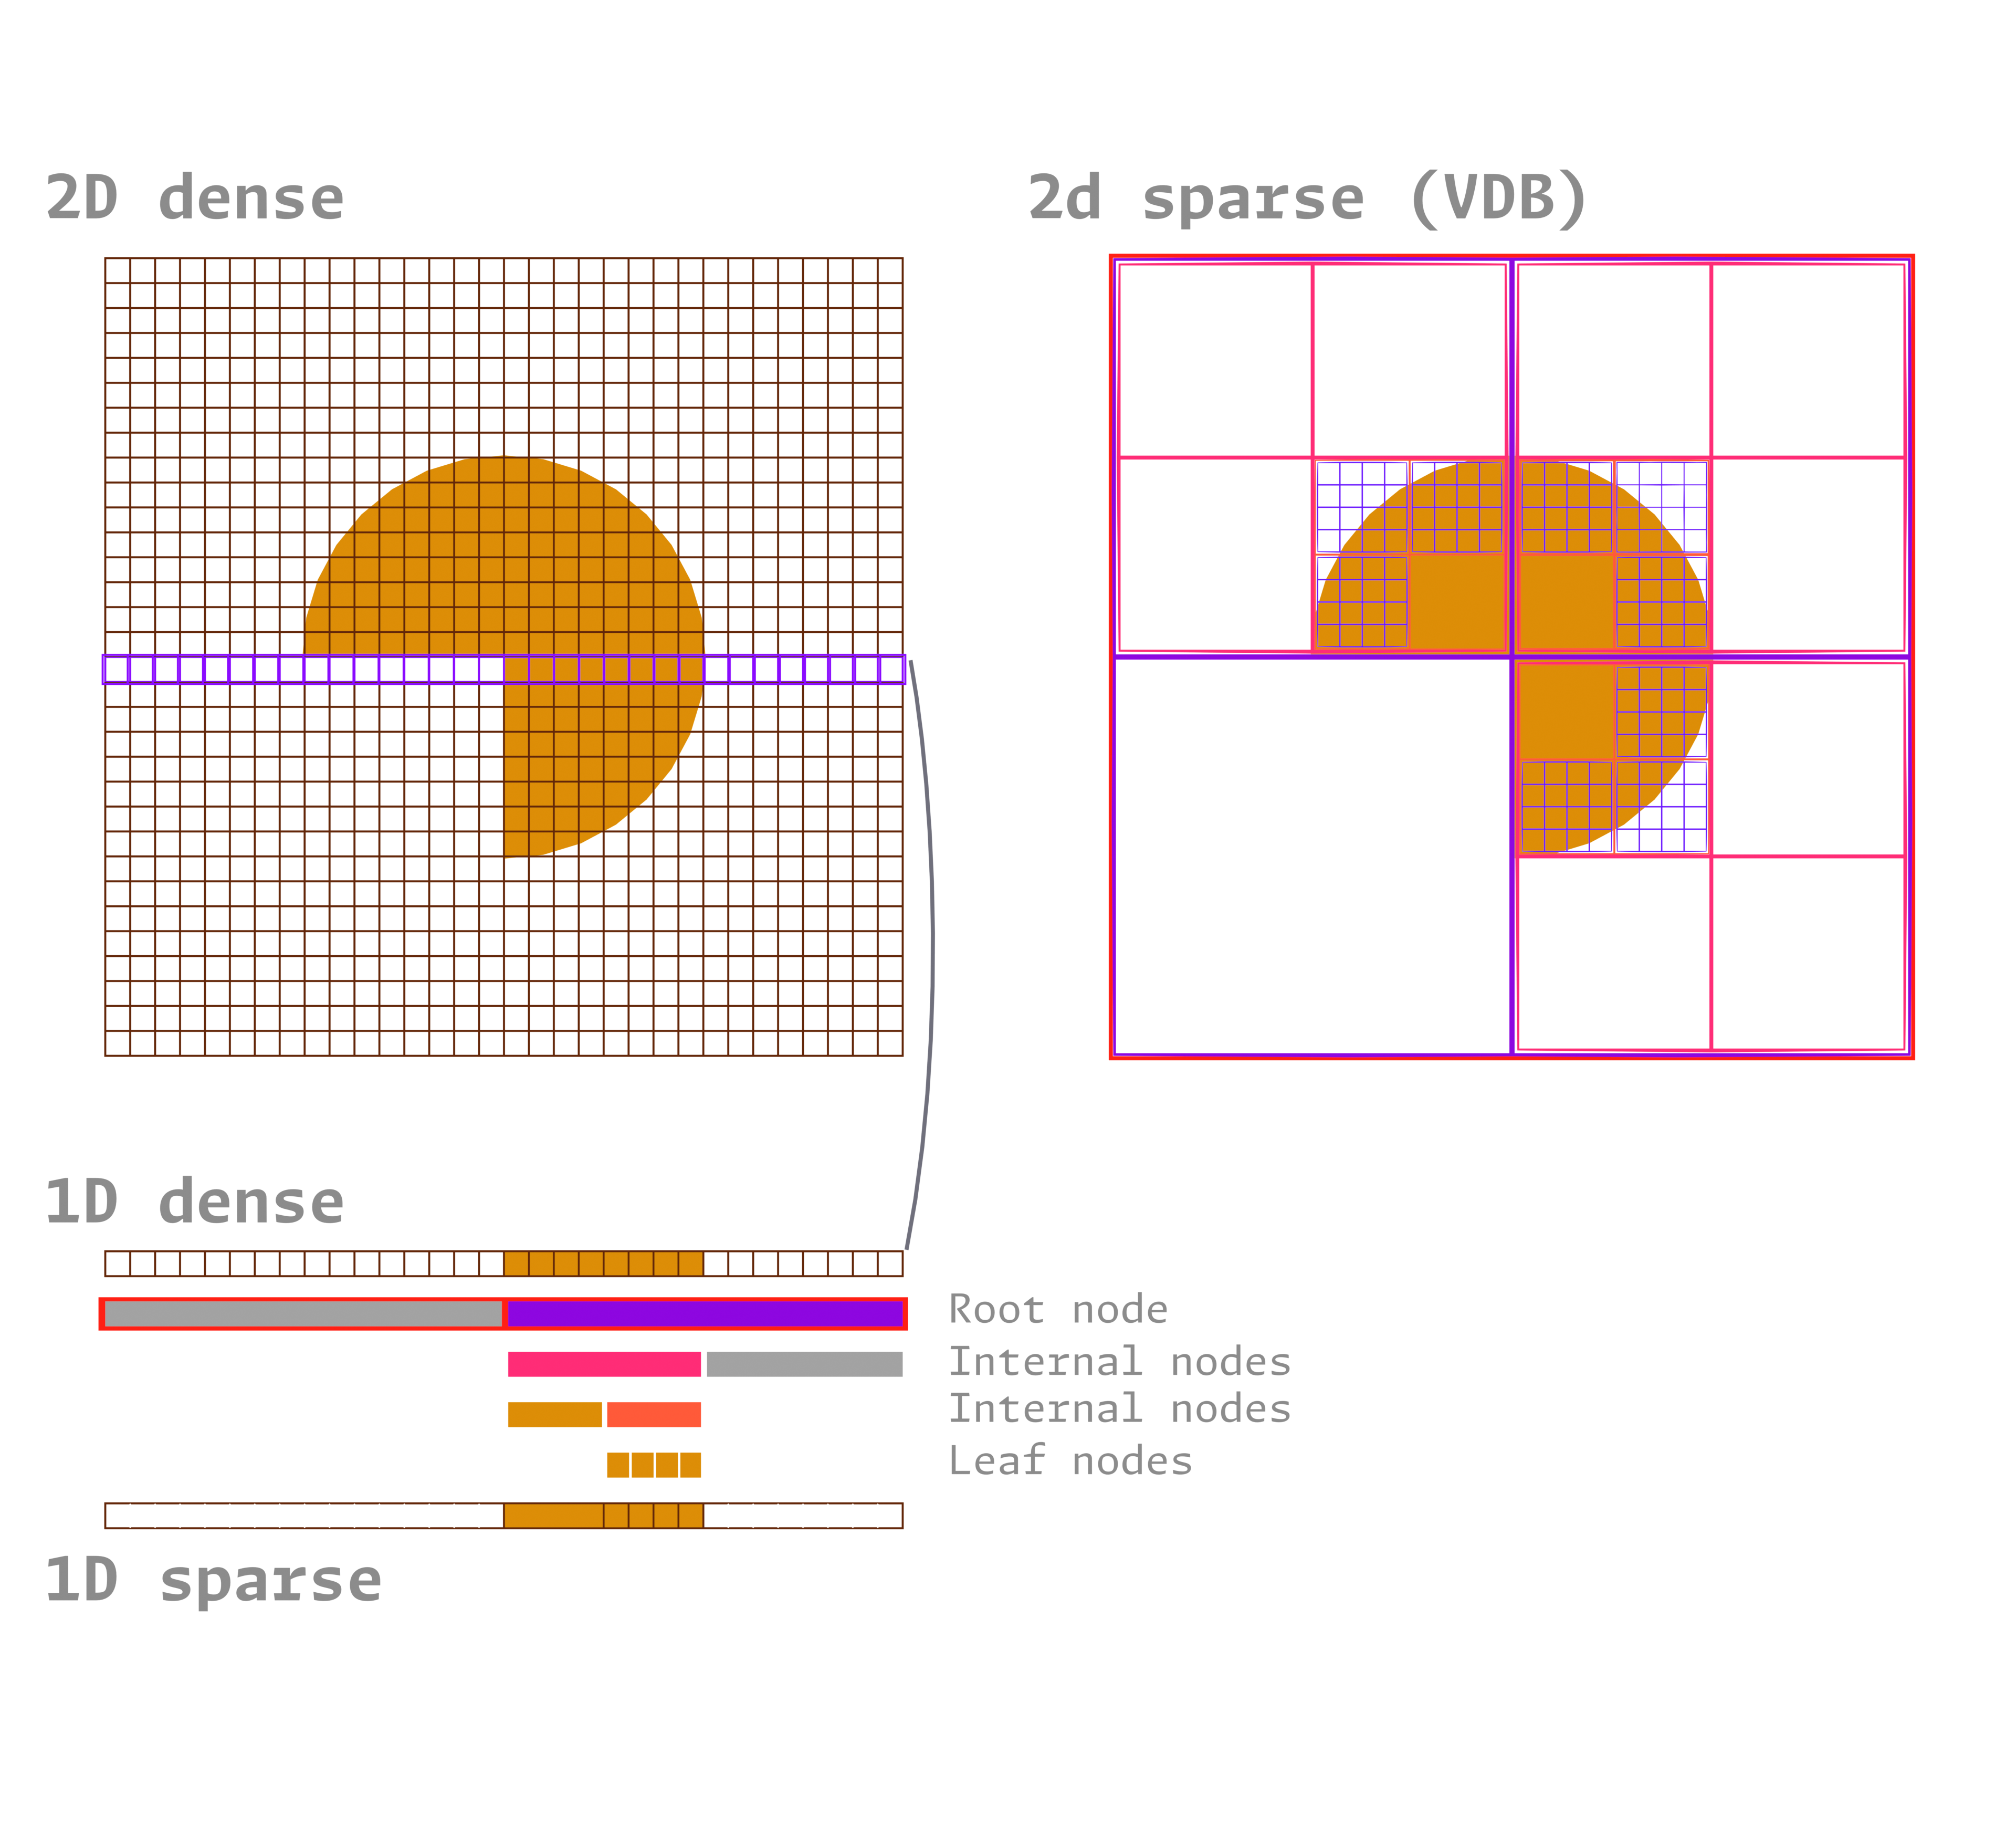
\includegraphics[width=\linewidth]{vdb}
  \caption{2D \& 1D slices of the VDB data structure representing three quarters of a circle. Top left: 2D dense representation of the circle. Top right: 2D sparse representation of the VDB. Bottom left: Sparse representation of the 1D vdb. Usually, VDB nodes have many more child nodes, which whould make it harder to visualise, hence a smaller version of VDB is shown. This figure is an augumented version of the one in the original paper\supercite{vdb2013}}
\end{figure}

At the hear of the data structure are its three types of nodes, internal root and leaf. The VDB data structure is inherently general, each of the nodes' sizes can be modefied depending on the application. However, in practice only one specialization of the VDB structure is used, that is the VDB345. This is because the authors of the original paper\supercite{vdb2013} analyized a suite of possible shapes and sizes, and this configuration of VDB the most balanced between performance and memory footprint for most practical applications [TODO: what applications?]

\paragraph{Leaf Nodes} They are the lowest level in the tree structure. They store a 3D cubed grid of side length $2^{\log_{2} D}$ (i.e. only powers of 2). An leaf value in the grid can be a voxel's data, other associated data for empty values (such as SDF information), or an empty value.
Leaf nodes also store a value mask. This is a bit-array meant to compactly determine if value at a specific coordinate in the 3D grid is voxel data or an empty value.

In the implementation the trait \verb|Node| is defined which gives some associated data and methods leaf and internal nodes have.

\begin{lstlisting}[language=rust,caption={\texttt{Node} trait definition},captionpos=b,label={code:node}]
pub trait Node {
    /// LOG2_D of side length
    /// LOG2_D = 3 => `512 = 8 * 8 * 8` values
    const LOG2_D: u64;
    /// Total conceptual LOG2_D node
    const TOTAL_LOG2_D: u64;
    /// Total conceptual LOG2_D of child node
    const CHILD_TOTAL_LOG2_D: u64 = Self::TOTAL_LOG2_D - Self::LOG2_D;
    /// Side length
    const DIM: u64 = 1 << Self::LOG2_D;
    /// Total conceptual dimension
    const TOTAL_DIM: u64 = 1 << Self::TOTAL_LOG2_D;
    /// Size of this node (i.e. length of data array)
    const SIZE: usize = 1 << (Self::LOG2_D * 3);
    /// Total conceptual size of node, including child size
    const TOTAL_SIZE: u64 = 1 << (Self::TOTAL_LOG2_D * 3);
}
\end{lstlisting}

In \cref{code:node}, \verb|TOTAL_LOG2_D| represents the $\log_{2}$ of the total dimension of the node, meaning how much actual space the node occupies. Leaf nodes are at the bottom of the tree and don't have children so this is the same as $\log_{2} D$, but this value will be relevant for internal nodes. All other attributes are determined at compile-time depending on the size of the node $\log_{2} D$.

\begin{quote}
  \paragraph{Sidenote on Coordinate Systems}

  It is very convenient for side lengths to be powers of two because of the way integers are stored in memory, as binary values. To get the global coordinate of a node with \verb|TOTAL_LOG2_D| $= 3$ that contains a point in global coordinates, the 3 least signifcant bits of each coordinate have to be masked out. This can essentially be done in a single CPU instruction for each coordinate.

\begin{lstlisting}[language=rust]
/// Give global origin of Node coordinates from `global` point
fn global_to_node(global: GlobalCoordinates) -> GlobalCoordinates {
    global.map(|c| (c >> Self::TOTAL_LOG2_D) << Self::TOTAL_LOG2_D)
}
\end{lstlisting}

Simillary, to get the relative coordinates of a global point within the node are precisely the \texttt{TOTAL\_LOG2\_D} least siginificant bits.

\begin{lstlisting}[language=rust]
/// Give local coordinates relative to the Node containing `global` position
fn global_to_relative(global: GlobalCoordinates) -> LocalCoordinates {
    global.map(|c| (c & ((1 << Self::TOTAL_LOG2_D) - 1)))
}
\end{lstlisting}

This pattern of a few bit-wise operations can acheive any conversion from between coordinate systems one might need, and all of these through operations are extremly fast to compute on modern CPUs.
\end{quote}

\Cref{code:leaf} shows a simplified definition of the leaf node data structure in the implementation. It has two fields: data which is an array representing the 3D cube grid of values, and value mask which is a the bit-mask carrying information on what each value represnts, a voxel or empty space. the data array has has $2^{3\log_{2} D}$ entries(e.g. for $\log_{2} D = 3 \Rightarrow D = 8$ the leaf node has $8\times8\times8 = 512 = 2^{9}$ values). The value mask has the same number of bit entries, but it is stored as an array of unsined 64 bit integers, hence there are $\frac{D^{3}}{64}$ of them.

\begin{lstlisting}[language=rust, captionpos=b, caption={
    \texttt{LeafNode} definition.
    In the original paper\supercite{vdb2013} node data is set as a union instead of a enum, in order to save on memory space, only using the masks to determine the type of a particular values.
    In this implementation a enum is used strictly for \emph{ergonomics}, as the extra 1 byte of memory per value is generally not expensive on heap allocated memory.
    The value mask will still be curcial for the GPU version of VDB where there is more need for effective memory management and shading languages do not have enum support.
    In the \texttt{Node} trait implementation, since these nodes are the bottom level in the hierarchy (meaning they have no children), their in-memory dimensions are the same as their world space dimensions.
  }, label{code:leaf}]
pub struct LeafNode<ValueType, const LOG2_D: u64>
{
    pub data: [LeafData<ValueType>; (1 << (LOG2_D * 3))],
    pub value_mask: [u64; ((1 << (LOG2_D * 3)) / 64)],
}

pub enum LeafData<ValueType> {
    Tile(usize),
    Value(ValueType),
}

impl<ValueType, const LOG2_D: u64> Node for LeafNode<ValueType, LOG2_D>
{
    const LOG2_D: u64 = LOG2_D;
    const TOTAL_LOG2_D: u64 = LOG2_D;
}
\end{lstlisting}

The implenetation is general both in the type of value that is stored at the voxel level, \verb|ValueType|, and in the dimension of the Node, \verb|LOG2_D|. This makes use of Rust's generic const expresions feature \supercite{rust:generic} that is only available on the nightly toolchain. These work in a way akin to C++ templates allowing to define types of static size chosen by the user of the data structure that are resolved at compile time. This approach effectively allows to costumize the tree breadth and depth at compile time with no run-time overhead.

\paragraph{Internal Nodes} They sit between the root node and the leaf nodes, forming the middle layer of the tree structure.
They also store a 3D cubed grid of side length $2^{D}$ of values. An internal value can either be a pointer to a child node (leaf or internal), or a tile value, which is a value that is the same for the whole space that would be covered by a child node in that position.
Internal nodes also store a value mask and child mask. These determine if value at a specific coordinate in the 3D grid is child pointer, value type or empty value.


\begin{lstlisting}[language=rust, captionpos=b, caption={
    \texttt{InternalNode} definition. Internal nodes have an extra field, the child mask that is the same size of the value mask.
    Aditionally the internal data enum now has variants for a child pointer or 4 bytes of memory.
}]
pub struct InternalNode<ValueType, ChildType: Node, const LOG2_D: u64>
{
    pub data: [InternalData<ChildType>; (1 << (LOG2_D * 3))],
    pub value_mask: [u64; ((1 << (LOG2_D * 3)) / 64)],
    pub child_mask: [u64; ((1 << (LOG2_D * 3)) / 64)],
}

pub enum InternalData<ChildType> {
    Node(Box<ChildType>),
    Tile(u32),
}

impl<ValueType, ChildType: Node, const LOG2_D: u64> Node
    for InternalNode<ValueType, ChildType, LOG2_D>
{
    const LOG2_D: u64 = LOG2_D;
    const TOTAL_LOG2_D: u64 = LOG2_D + ChildType::TOTAL_LOG2_D;
}
\end{lstlisting}

When implemening the \verb|Node| the \verb|TOTAL_LOG2_D| is calculated by adding this nodes $\log_{2}D$ with the child node's total $\log_{2}D$.
For example, for an internal node with $log_{2}D = 4$ with children that are leaf nodes of $log_{2}D' = 3$, the internal node's $\log_{2}D_{{total}}$ will be $7$. This means that the internal node has $16\times16\times16$  children that each have $8\times8\times8$ voxels; the total number of voxels one of these internal nodes is $128\times128\times128$ or $2^{7}\times2^{7}\times2^{7}$.

It is imporant to note that all children of an internal node must be of the same type, which means each level in the tree only has one type of node, this ensure consistency in the coordinate system discussed previously.

\paragraph{Root Node} The root node is a single node at the top of the VDB hierarchy. Unlike typical nodes in a tree data structure, the root node in a VDB does not store data directly but instead serves as an entry point to the tree.
It contains a hash map indexed by global coordinates, linking to all its child nodes. This setup allows for quick access and updates, as the root node acts as a guide to more detailed data stored deeper in the hierarchy. Because its children nodes are stored by a hash map, it only stores information about space that has information to be stored(unlinke an octree where empty top level nodes are frequent). The root node's primary role is to organize and provide access to internal nodes.


\begin{lstlisting}[language=rust, captionpos=b, caption={
    \texttt{RootNode} definition. \texttt{RootData} is either a pointer to a child or a 4 bytes of data for a tile value.
  },label={code:root}]
pub struct RootNode<ValueType, ChildType: Node>
{
    pub map: HashMap<GlobalCoordinates, RootData<ChildType>>,
}

pub enum RootData<ChildType> {
    Node(Box<ChildType>),
    Tile(u32),
}
\end{lstlisting}

Finally, a VDB simply consits of a root node and some metadata associated with the volume, stored in the \verb|grid_descriptor| feild. This metadata is generally only imprtant when reading enad writing \verb|.vdb| files.

\begin{lstlisting}[language=rust, captionpos=b, caption={\texttt{VDB} definition}]
pub struct VDB<ValueType, ChildType: Node>
{
    pub root: RootNode<ValueType, ChildType>,
    pub grid_descriptor: GridDescriptor,
}
\end{lstlisting}

\subsubsection{VDB345}
$\rm{VDB}345$ is the most widely used configuration of the VDB data structure, because gives a good balance of performance and memory footprint for most applications.
\begin{sloppypar}
  To refer to different shapes of the VDB data structure, by convention, they are named as ${\rm{VDB}[a_{0},a_{1},\dots, a_{n}]}$, meaning it has a  bottom layer of leaf nodes with $\log_{2}D_{0}=a_{0}$ follwed by $n$ layers of internal nodes with $\log_{2}D_{i}=a_{i}$. $\rm{VDB}345$ therfore with leaf nodes with $\log_{2}D_{n3} = 3$ and two layers of internal nodes, one with $\log_{2}D_{n4} = 4$ and the other with $\log_{2}D_{n5} = 5$.
\end{sloppypar}

To implement this type of VDB new type name for each type of node is created as show in \cref{vdb345}, chaining them up the tree. This section will refer to these nodes as \texttt{Node3}s, \texttt{Node4}s and \texttt{Node5}s respectively.

\begin{lstlisting}[language=rust, captionpos=b, caption={\texttt{VDB345} definition}, label={vdb345}]
pub type N3<ValueType> = LeafNode<ValueType, 3>;
pub type N4<ValueType> = InternalNode<ValueType, N3<ValueType>, 4>;
pub type N5<ValueType> = InternalNode<ValueType, N4<ValueType>, 5>;
pub type VDB345<ValueType> = VDB<ValueType, N5<ValueType>>;
\end{lstlisting}

To calculate how much the in-memory size, in bytes, of each node the follwing calculation can be done, by taking into account the size of the 3D grid together with the masks:
\begin{align*}
&\text{For leaf nodes:}& M &= D^{3} (v + 1) + \frac{D^{3}}{8} \\
&\text{For internal nodes (2 masks):}& M &= D^{3} (v + 1) + 2\frac{D^{3}}{8} \\
&\text{Where:}& D &= \text{dimension of node (side-length)} \\
&& v &= \text{number bytes the value type occupies (min. of 4)}
\intertext{Simillarly to find out how many voxels each node covers in world space:}
  &\textbf{Node3:}& D &= 2^3 = 8 \\
  && S &= D^3 = 8\times8\times8 = 512 \\
  &\textbf{Node4:}& D &= 2^4 = 16 \\
  && D_{t} &= 2^{4+3} = 128 \\
  && S &= D_{t}^3 = 128\times128\times128 = 2,097,152 \\
  &\textbf{Node5:}& D &= 2^5 = 32 \\
  && D_{t} &= 2^{5+4+3} = 4096 \\
  && S &= D_{t}^3 = 4096\times4096\times4096 = 68,719,476,736
\end{align*}

A single Node5 represent $4069^3$ voxels in space, just under $69$ billion.
This is where the power of the VDB data structure can be seen; models can have multiple \verb|Node5|s covering trillions of voxels in total all of which can be acessed in $O(1)$ time, by going three layers down the tree.


\subsubsection{Reading \texttt{.vdb}}
VDB was introduced along with an associated file format \verb|.vdb| which gives a compact representation of the data structure. In this section the part of the implementatio that reads VDB files and stores them into memory is covered.

\subsubsection{Computing SDF}
\subsubsection{GPU VDB}
